\documentclass[11pt]{article}
\usepackage[T1]{fontenc}
\usepackage{lmodern}
\usepackage[margin=1in]{geometry}
\usepackage{amsmath,amssymb,amsthm,mathtools,booktabs,graphicx}
\usepackage{microtype}
\usepackage{enumitem}
\usepackage[hidelinks]{hyperref}
\hypersetup{pdftitle={Historic tree asymptotics and a high order obstruction},pdfauthor={},pdfsubject={Reduced historic trees; low-order asymptotics and a counterexample to the general coefficient conjecture}}
\setlength{\emergencystretch}{2em}
\setlength{\belowcaptionskip}{6pt}
\setlist{itemsep=3pt,topsep=5pt}
\newtheorem{theorem}{Theorem}[section]
\newtheorem{proposition}[theorem]{Proposition}
\newtheorem{lemma}[theorem]{Lemma}
\newtheorem{corollary}[theorem]{Corollary}
\theoremstyle{remark}\newtheorem{remark}[theorem]{Remark}
\DeclareMathOperator{\Rea}{Re}
\DeclareMathOperator{\Ima}{Im}
\DeclareMathOperator{\Log}{Log}
\newcommand{\dd}{\,\mathrm d}
\newcommand{\eps}{\varepsilon}
\newcommand{\C}{\mathbb C}
\newcommand{\R}{\mathbb R}
\newcommand{\N}{\mathbb N}
\newcommand{\la}{\lambda}
\newcommand{\lab}{{\overline{\lambda}}}
\numberwithin{equation}{section}
\title{Historic tree asymptotics\\and a high order obstruction}
\author{Research article and reproducibility report}
\date{2 October 2026}
\begin{document}
\maketitle
\begin{abstract}
For the all-one family $H_r^{(r)}=H_r^2$, we prove the $m=2$ and $m=3$ instances of Burghart and Wagner's 2026 historic-tree coefficient conjecture, where $r=m+1$, and disprove every instance with $m\ge29$ for the specified counting sequences. For reduced $5$- and $7$-historic trees, the respective equivalents are $30(n+2)!\rho_3^{-n-3}$ and $140(n+3)!\rho_4^{-n-4}$. Both have rigorously nonzero corrections oscillating in $\log n$, convergent local complex-power expansions, all fixed coefficient grades with exact Gamma ratios, and qualified eventual inverse brackets. Astashova's earlier real-axis blowup laws are credited. For every ODE order $r\ge30$, an elementary spectral estimate and a closed sign-variation cone exclude convergence of the actual all-one orbit to the normalized pole equilibrium. Exact rational certificates cover the finite bridge at orders $30$ through $37$. The spectrum itself has antecedents in B-urns and higher-order Emden--Fowler theory; the obstruction uses the specific initial data. Exact checks and replayable certificates are separated from non-certified numerical illustrations. No replacement high-order asymptotic or periodic limiting profile is asserted.
\end{abstract}
\setcounter{tocdepth}{1}
{\small\tableofcontents}
\newpage

\section{The counting problem and the results}
\subsection{The published target}
Burghart and Wagner's model of reduced $(2m+1)$-historic trees has exponential generating function
\begin{equation}\label{eq:family}
 H^{(m+1)}=H^2,\qquad H^{(j)}(0)=1\quad(0\le j\le m).
\end{equation}
A reduced tree of size $n$ corresponds to a B-tree history of length $n+m$. Their Conjecture~1 predicts
\begin{equation}\label{eq:conjecture}
 h_n\sim\frac{(2m+1)!}{(m!)^2}(n+m)!\rho_m^{-n-m-1}.
\end{equation}
The journal statement appears in Section~4 of \cite{bw2026}; its predecessor is Conjecture~10 of \cite{bw2024}. The detailed argument in Sections~2--7 addresses $m=2$, for which
\begin{equation}\label{eq:ivp}
 H'''(z)=H(z)^2,\qquad H(0)=H'(0)=H''(0)=1.
\end{equation}
Equating exponential coefficients gives
\begin{equation}\label{eq:recurrence}
 h_0=h_1=h_2=1,\qquad
 h_{n+3}=\sum_{j=0}^n\binom njh_jh_{n-j},\qquad
 H(z)=\sum_{n\ge0}h_n\frac{z^n}{n!}.
\end{equation}
This recurrence identifies the sequence with OEIS A333497 \cite{oeis}. The identification is by recurrence; it is not an assertion that the journal paper names this OEIS entry. The beginning is
\[
1,1,1,1,2,4,8,18,48,144,456,1560,5808,23184,98160,440832.
\]

\subsection{The conclusions across orders}
Two low-order instances hold, but the conjecture as stated for all orders is false. ODE order $r$ equals $m+1$; the historic-tree order is $2m+1$.
\begin{center}
\begin{tabular}{c c l}
\toprule
$m$ & $r$ & Conclusion for the all-one sequence\\
\midrule
2 & 3 & A333497: equivalent, nonzero oscillation, all fixed grades\\
3 & 4 & A336009: equivalent, nonzero oscillation, all fixed grades\\
$\ge29$ & $\ge30$ & Every corresponding proposed equivalent is false\\
\bottomrule
\end{tabular}
\end{center}
The first two cases also admit eventual inverse brackets. Their real-axis leading powers use or recover Astashova's prior results; the coefficient conclusions require complex continuation. The last case is an obstruction for the specified initial jet, rather than an inference from generic instability. We first establish the third-order case in full detail and then isolate the additional arguments needed for the fourth-order result and the uniform high-order obstruction.

\subsection{The third order theorem}
Throughout, powers of $t=\rho-z$ use a logarithm that is real on $t>0$. Put
\begin{equation}\label{eq:exponents}
 \la=\frac{13+i\sqrt{71}}2,\qquad
 \lab=\frac{13-i\sqrt{71}}2,\qquad
 \alpha=\frac{13}{2},\quad \omega=\frac{\sqrt{71}}2,\quad
 \nu_{kl}=k\la+l\lab.
\end{equation}
A \emph{grade} means the total degree $k+l$ in the two local complex powers. It is held fixed when $n\to\infty$.

\begin{theorem}[Counting asymptotics and convergent local expansion]\label{thm:main}
The solution of \eqref{eq:ivp} has a finite positive blowup point $\rho$, satisfying
\begin{equation}\label{eq:rho-bounds}
 180^{1/4}\le\rho\le60^{1/3}.
\end{equation}
Its Taylor series at zero has radius $\rho$, with no other singularity on $|z|=\rho$. There is a uniquely normalized $C\in\C\setminus\{0\}$ such that
\begin{equation}\label{eq:local}
 H(z)=60t^{-3}\mathcal F(Ct^\la,\overline C t^\lab),\qquad
 \mathcal F(X,Y)=\sum_{k,l\ge0}a_{kl}X^kY^l,
\end{equation}
where $\mathcal F$ is holomorphic in a bidisk at $(0,0)$,
\[
 a_{00}=a_{10}=a_{01}=1,\qquad a_{lk}=\overline{a_{kl}}.
\]
For each fixed finite angular interval on a chosen logarithmic sheet, \eqref{eq:local} converges for all sufficiently small $|t|$, uniformly on closed subsectors.

For every fixed integer $d\ge0$,
\begin{equation}\label{eq:count-theorem}
 \frac{h_n}{30(n+2)!\rho^{-n-3}}
 =Q_d(n)+O_d\bigl(n^{-\alpha(d+1)}\bigr),
\end{equation}
where, for all sufficiently large real $x$,
\begin{equation}\label{eq:Q}
 Q_d(x)=1+
 \sum_{\substack{1\le k+l\le d\\k\ne l}}
 \frac{2a_{kl}C^k\overline C^{\,l}\rho^{\nu_{kl}}}{\Gamma(3-\nu_{kl})}
 \frac{\Gamma(x+3-\nu_{kl})}{\Gamma(x+3)}.
\end{equation}
In particular, $h_n\sim30(n+2)!\rho^{-n-3}$.
\end{theorem}
The factor $2$ in each summand of \eqref{eq:Q} is present before conjugate pairing. Both $(k,l)$ and $(l,k)$ are included. All diagonal terms $k=l\ge1$ are excluded because they are analytic monomials at the singularity. The exact Gamma ratios preserve every integer inverse-$n$ correction belonging to a retained grade.

\begin{corollary}[A nonzero logarithmic oscillation]\label{cor:oscillation}
With
\begin{equation}\label{eq:K}
 K=\frac{2C\rho^\la}{\Gamma(3-\la)}\ne0,\qquad
 R_n=\frac{h_n}{30(n+2)!\rho^{-n-3}},
\end{equation}
one has
\begin{align}
 R_n&=1+2\Rea\left\{K\frac{\Gamma(n+3-\la)}{\Gamma(n+3)}\right\}
       +O(n^{-13}),\label{eq:first-exact}\\
 &=1+2|K|n^{-13/2}\cos(\arg K-\omega\log n)
       +O(n^{-15/2}).\label{eq:first-simple}
\end{align}
Consequently,
\begin{equation}\label{eq:limsup}
 \limsup_{n\to\infty}n^{13/2}(R_n-1)=2|K|,
 \qquad
 \liminf_{n\to\infty}n^{13/2}(R_n-1)=-2|K|.
\end{equation}
The error $R_n-1$ changes sign infinitely often and is not $O(n^{-7})$.
\end{corollary}

\subsection{Attribution and the logical route}
Astashova's Theorem~3 \cite{astashova2013} already gives the real-axis law
$H(x)\sim60(\rho-x)^{-3}$ for positive blowup solutions of this third-order equation. Her theorem covers orders $3$ and $4$ under the stated Emden--Fowler hypotheses; it is not a theorem for all orders. The self-contained real argument below also proves finite blowup for our selected initial data. It is an alternate derivation, not a claim of priority for the real-axis law.

Real-axis blowup alone does not justify individual coefficient asymptotics. The remaining work is to obtain a convergent holomorphic local representation, prove that the first complex amplitude cannot vanish, exclude competing singularities on the convergence circle, and establish a domain in which singularity analysis applies. Holomorphic Poincar\'e linearization \cite{iy2008}, Pringsheim's theorem, and the standard transfer theorems \cite{fs2009} are used in their usual forms. The fourth-order extension and the high-order obstruction follow in Sections~\ref{sec:r4} and \ref{sec:obstruction}. The arguments are conventional analytic proofs accompanied by exact checks, not proof-assistant formalizations.

\section{A global real solution and finite blowup}
\subsection{Desingularization}
For a positive solution set
\begin{equation}\label{eq:coordinates}
 p=H'H^{-4/3},\qquad q=H''H^{-5/3},\qquad
 \frac{\dd\tau}{\dd x}=H^{1/3}.
\end{equation}
Direct differentiation gives the autonomous planar system
\begin{equation}\label{eq:planar}
 \dot p=q-\frac43p^2,\qquad
 \dot q=1-\frac53pq,\qquad (p(0),q(0))=(1,1),
\end{equation}
where dots mean $\tau$ derivatives. Its positive quadrant is forward invariant: on $p=0$ the first component equals $q>0$, and on $q=0$ the second equals $1>0$. The unique positive equilibrium is
\begin{equation}\label{eq:equilibrium}
 p_*=(9/20)^{1/3},\qquad q_*=\frac43p_*^2,
 \qquad p_*q_*=\frac35.
\end{equation}

\begin{lemma}[Strict Lyapunov dissipation]\label{lem:lyapunov}
On $p\ge0$, $q>0$, let
\begin{equation}\label{eq:V}
 V(p,q)=\frac56(p-p_*)^2+q-q_*-q_*\log(q/q_*).
\end{equation}
Then $V\ge0$, vanishing only at the equilibrium, and
\begin{equation}\label{eq:Vdot}
 \dot V=-\frac{20}{9}(p-p_*)^2(p+p_*)
        -\frac53p_*\frac{(q-q_*)^2}{q}.
\end{equation}
The orbit in \eqref{eq:planar} exists for every $\tau\ge0$ and converges to $(p_*,q_*)$.
\end{lemma}
\begin{proof}
Write $A=4/3$ and $B=5/3$. At the equilibrium,
\[
 \dot p=(q-q_*)-A(p^2-p_*^2),\qquad
 \dot q=-B\{q(p-p_*)+p_*(q-q_*)\}.
\]
Multiply these equations by $B(p-p_*)$ and $1-q_*/q$, respectively. Their cross terms cancel, giving \eqref{eq:Vdot}. The logarithmic term in $V$ tends to infinity both as $q\downarrow0$ and as $q\to\infty$; the quadratic term bounds $p$ above. Thus the orbit stays in a compact sublevel in $p\ge0$, $q>0$. Such a set may meet $p=0$, but the polynomial vector field is regular there and points inward. This causes no loss of continuation.

On this sublevel, \eqref{eq:Vdot} bounds the integrals of $(p-p_*)^2$ and $(q-q_*)^2$. Their derivatives are bounded, hence the squared deviations are uniformly continuous. A nonnegative uniformly continuous integrable function tends to zero: otherwise separated intervals of fixed positive area contradict integrability. Applying this observation twice proves convergence. Equivalently, LaSalle's invariance principle applies because the zero set of \eqref{eq:Vdot} is a single point.
\end{proof}

\subsection{Reconstruction of the original time}
The construction can be reversed without any blowup assumption. Define
\begin{equation}\label{eq:reconstruction}
 H(\tau)=\exp\!\left(\int_0^\tau p(s)\dd s\right),\qquad
 x(\tau)=\int_0^\tau H(s)^{-1/3}\dd s.
\end{equation}
For $x=x(\tau)$, direct differentiation using \eqref{eq:planar} verifies \eqref{eq:ivp} and its initial data. Since $p(\tau)\to p_*>0$, $H$ grows exponentially in $\tau$, and
\begin{equation}\label{eq:rho}
 0<\rho:=\int_0^\infty H(s)^{-1/3}\dd s<\infty.
\end{equation}
Thus $x(\tau)\uparrow\rho$ and $H(x)\to\infty$. No earlier real obstruction occurs.

Put $v=H^{-1/3}$. In the original variable,
\begin{equation}\label{eq:vprime}
 v'(x)=-\frac{p(x)}3,\qquad
 v(x)=\frac13\int_x^\rho p(s)\dd s
 \sim\frac{p_*}3(\rho-x).
\end{equation}
Here $p(x)$ means $p(\tau(x))$. It follows that
\begin{equation}\label{eq:real-leading}
 H(x)\sim\left(\frac3{p_*}\right)^3(\rho-x)^{-3}
       =60(\rho-x)^{-3}.
\end{equation}
All three components required in Astashova's real-axis hypotheses diverge, since $p\to p_*>0$ and $q\to q_*>0$.

\subsection{Analytic bounds for the radius}
The rectangle
\begin{equation}\label{eq:rectangle}
 \frac35\le p\le1,\qquad \frac{12}{25}\le q\le1
\end{equation}
is forward invariant and contains $(1,1)$. On its four faces,
\[
 \dot p\big|_{p=3/5}=q-12/25\ge0,\quad
 \dot p\big|_{p=1}\le-1/3,\quad
 \dot q\big|_{q=12/25}=1-4p/5\ge1/5,\quad
 \dot q\big|_{q=1}\le0.
\]
Integrating \eqref{eq:vprime} gives the useful tail bounds
\begin{equation}\label{eq:tail-bounds}
 x+3H(x)^{-1/3}\le\rho\le x+5H(x)^{-1/3}
 \qquad(0\le x<\rho).
\end{equation}
At zero these imply $3<\rho<5$, with strictness because $p$ is not identically an endpoint.

A tighter initial bound comes from the exact pole solutions
\[
 P_s(x)=60(s-x)^{-3},\qquad
 (P_s(0),P_s'(0),P_s''(0))=(60s^{-3},180s^{-4},720s^{-5}).
\]
For $s=180^{1/4}$ this initial vector dominates $(1,1,1)$ componentwise; for $s=60^{1/3}$ it is dominated by $(1,1,1)$. The system
\[
 (H,H',H'')'=(H',H'',H^2)
\]
is cooperative in the nonnegative octant. Its comparison principle, up to the first blowup of either solution, therefore yields \eqref{eq:rho-bounds}. Numerically, only for orientation,
\[
 3.66284150148\ldots\le\rho\le3.91486764116\ldots.
\]
These bounds are analytic and independent of every fitted value below.

\section{A convergent expansion at the singularity}
\subsection{Holomorphic linearization}
The Jacobian of \eqref{eq:planar} at the equilibrium is
\begin{equation}\label{eq:jacobian}
 A=\begin{pmatrix}-8p_*/3&1\\-5q_*/3&-5p_*/3\end{pmatrix},\qquad
 \det(\mu I-A)=\mu^2+\frac{13p_*}{3}\mu+\frac{20p_*^2}{3}.
\end{equation}
Its eigenvalues are $p_*(-13\pm i\sqrt{71})/6$. Put
\begin{equation}\label{eq:a}
 a=\frac{p_*}3=60^{-1/3}.
\end{equation}
Label the eigenvalues $-a\la$ and $-a\lab$. Their convex hull excludes zero. A resonance of degree $k+l\ge2$ would require
$k(-a\la)+l(-a\lab)$ to equal one eigenvalue; equality of real parts would force $k+l=1$. Thus no resonance exists.

The holomorphic Poincar\'e linearization theorem \cite{iy2008} gives holomorphic coordinates $u_+,u_-$ near the equilibrium with
\begin{equation}\label{eq:linearization}
 \dot u_+=-a\la u_+,\qquad \dot u_-=-a\lab u_-,\qquad
 p=p_*+P(u),\quad P(u)=u_++u_-+O(\|u\|^2).
\end{equation}
Every eigenvector of $A$ has a nonzero first component, so this normalization is possible. Choose conjugate eigenvectors; uniqueness of the normalized nonresonant conjugacy then preserves the real structure. Along our real orbit, $u_- =\overline{u_+}$.

\subsection{Removing the multiplicative correction}
The variable $v=H^{-1/3}$ satisfies
\begin{equation}\label{eq:vdot}
 \dot v=-\bigl(a+P(u)/3\bigr)v.
\end{equation}
Let $\mathcal L=\la u_+\partial_{u_+}+\lab u_-\partial_{u_-}$. The homological equation
\begin{equation}\label{eq:S}
 \mathcal L S=-P/p_*,\qquad S(0)=0
\end{equation}
has the unique holomorphic solution
\[
 S_{kl}=-\frac{P_{kl}}{p_*(k\la+l\lab)}\quad(k+l\ge1).
\]
Indeed, the real part of each denominator apart from $p_*$ is $\alpha(k+l)$, so division preserves convergence of the power series. Now
\begin{equation}\label{eq:w}
 w=v\exp S(u)\quad\Longrightarrow\quad \dot w=-aw.
\end{equation}
For a sufficiently late point on the real orbit, $w>0$ and
\begin{equation}\label{eq:constants}
 u_+=K_+w^\la,\qquad u_-=K_-w^\lab,\qquad K_- =\overline{K_+}.
\end{equation}
If either constant vanished, both would vanish, making the local orbit the equilibrium. Uniqueness would then make the whole planar orbit the equilibrium, contradicting $(p(0),q(0))=(1,1)$. Hence both constants are nonzero.

Let $E(u)=\exp[-S(u)]$ and define
\begin{equation}\label{eq:Btime}
 B(u)=\sum_{k,l\ge0}\frac{E_{kl}}{1+k\la+l\lab}u_+^ku_-^l.
\end{equation}
Again the denominators preserve convergence; $B(0)=1$ and $(1+\mathcal L)B=E$. The remaining original time is exactly
\begin{equation}\label{eq:time-exact}
 t=\rho-x=\int_\tau^\infty v(s)\dd s=\frac{w}{a}B(u).
\end{equation}
For example, differentiating the right-hand side gives $-wE=-v$, and its limit at infinity is zero. This proves the identity without a merely formal integration.

\subsection{Analytic inversion and a nonzero linear term}
Set $\eta_+=K_+(at)^\la$, $\eta_-=K_-(at)^\lab$ and seek $w=at\mathcal R(\eta)$. Equation \eqref{eq:time-exact} becomes
\begin{equation}\label{eq:implicit}
 \mathcal R\,B\bigl(\eta_+\mathcal R^\la,\eta_-\mathcal R^\lab\bigr)=1.
\end{equation}
Powers of $\mathcal R$ use the holomorphic logarithm near $1$. At $(\mathcal R,\eta)=(1,0)$ the derivative with respect to $\mathcal R$ equals $1$. The analytic implicit-function theorem gives a unique holomorphic $\mathcal R$ with $\mathcal R(0)=1$. Therefore
\begin{align}
 H&=60t^{-3}F(\eta),\label{eq:Fraw}\\
 F(\eta)&=\mathcal R(\eta)^{-3}
 \exp\!\left[3S\bigl(\eta_+\mathcal R(\eta)^\la,
                         \eta_-\mathcal R(\eta)^\lab\bigr)\right].\nonumber
\end{align}
This is a holomorphic function of two independent variables near zero.

The linear coefficients, with $e_j$ denoting a coordinate multi-index, are
\begin{equation}\label{eq:linearcoeff}
 S_{e_j}=-\frac1{p_*\la_j},\qquad
 B_{e_j}=\frac1{p_*\la_j(1+\la_j)},\qquad
 F_{e_j}=-\frac3{p_*(1+\la_j)},
\end{equation}
where $\la_+=\la$, $\la_-=\lab$. Thus
\begin{equation}\label{eq:Cnonzero}
 C=-\frac{3K_+a^\la}{p_*(1+\la)}\ne0.
\end{equation}
Absorbing these two nonzero linear coefficients into the arguments of $F$ produces exactly the normalization $\mathcal F$ in \eqref{eq:local}.

On every bounded interval of $\arg t$ on a logarithmic sheet,
\[
 |t^{\la_j}|=|t|^{13/2}\exp(-\Ima(\la_j)\arg t)\longrightarrow0.
\]
Hence the two-variable Taylor series converges throughout a sufficiently small corresponding sector. It agrees with the original solution along the positive real approach and therefore, by analytic uniqueness, on their common complex domain. The radius may shrink with the chosen angular interval; no radius uniform over arbitrarily many logarithmic sheets is claimed. In particular,
\begin{equation}\label{eq:first-local}
 H(z)=60t^{-3}\left(1+Ct^\la+\overline C t^\lab+O(|t|^{13})\right).
\end{equation}
The normalization and distinct exponents determine $C$ uniquely on the specified branch.

\section{Universal coefficients and analytic diagonal terms}
Substitution of \eqref{eq:local} into $H'''=H^2$ is justified by local convergence. For a monomial $t^{\nu-3}$, three $z$ derivatives multiply it by
$(3-\nu)(4-\nu)(5-\nu)$ and reduce its exponent by $3$. Isolating the two products with the constant term gives, for $k+l\ge2$,
\begin{equation}\label{eq:akl}
 D(\nu_{kl})a_{kl}
 =60\!\sum_{\substack{0\le i\le k,\ 0\le j\le l\\
                   (i,j)\ne(0,0),(k,l)}}a_{ij}a_{k-i,l-j},
\end{equation}
where
\begin{equation}\label{eq:D}
 D(\nu)=(3-\nu)(4-\nu)(5-\nu)-120
       =-(\nu+1)(\nu-\la)(\nu-\lab).
\end{equation}
This recurrence is universal: initial data select $\rho$ and $C$, whereas the normalized $a_{kl}$ depend only on the equation. All denominators at degree at least two are nonzero, because $\Rea\nu_{kl}\ge13$ whereas the roots of $D$ have real parts $-1$ and $13/2$. There are no logarithmic resonance terms in the local expansion.

For example,
\begin{align}
 a_{11}&=-\frac17,&
 a_{20}&=\frac{359+57i\sqrt{71}}{17978},\label{eq:first-coeffs}\\
 a_{30}&=\frac{-17559+4223i\sqrt{71}}{78725662},&
 a_{21}&=\frac{2571}{1312394}
           -\frac{42477i\sqrt{71}}{119427854}.\nonumber
\end{align}
The reflected coefficients are their conjugates. The code calculates and checks exact values through degree four and numerical values through degree six.

The diagonal is exceptional for coefficient transfer. If $k=l\ge1$, then
\begin{equation}\label{eq:diagonal}
 \nu_{kk}=13k,\qquad
 60a_{kk}|C|^{2k}t^{13k-3}
\end{equation}
is an analytic polynomial in $z$ of degree $13k-3$. Its $n$th Taylor coefficient is zero once $n>13k-3$. The convergent sum of the diagonal terms is an analytic \emph{local} background at $t=0$. Its local analyticity does not, by itself, give a global exponentially small error. For the fixed-grade theorem, only finitely many such polynomials need be removed, and their eventual contribution is exactly zero.

The indexing $(k,l)\mapsto\nu_{kl}$ is injective: its real and imaginary parts determine $k+l$ and $k-l$. Later, after integer inverse-$n$ corrections are introduced, different labels can have equal final exponents because $\la+\lab=13$. Such coefficients must be combined; the coincidence introduces no logarithms.

\section{The dominant circle and a transfer domain}
\subsection{Identification of the radius}
Write $H(z)=\sum_{n\ge0}b_nz^n$ to avoid confusing ordinary coefficients with $a_{kl}$. Then
\begin{equation}\label{eq:ordinary}
 b_0=b_1=1,\quad b_2=\frac12,\qquad
 b_{n+3}=\frac{\sum_{j=0}^nb_jb_{n-j}}{(n+1)(n+2)(n+3)}.
\end{equation}
Every $b_n$ is strictly positive. The radius $R$ of this Taylor series equals $\rho$. Indeed, real blowup implies $R\le\rho$. If $R<\rho$, Pringsheim's theorem would force a singularity at the positive point $R$, whereas analytic ODE continuation along the finite real solution makes $H$ regular there. This contradiction proves equality. The real solution and $\rho$ were established before this argument, so there is no circular definition.

\subsection{Strict majorization away from the positive point}
Fix $0<r<\rho$ and $\theta\notin2\pi\mathbb Z$. Each of $H,H',H''$ has strictly positive coefficients at all powers, including consecutive powers. Equality in the triangle inequality is therefore impossible, and
\begin{equation}\label{eq:strict}
 |H^{(j)}(re^{i\theta})|<H^{(j)}(r)\qquad(j=0,1,2).
\end{equation}
By continuity, choose one $0<\eps<r$ so that all three left sides are at most $H^{(j)}(r-\eps)$.

Let $z_0=re^{i\theta}$. The Taylor recurrence at $z_0$ has the same polynomial convolution form as \eqref{eq:ordinary}. Its first three coefficients, after taking absolute values, are bounded by those of $H(r-\eps+w)$. Induction in the recurrence gives coefficientwise domination at every degree. The real-centered comparison series has nonnegative coefficients and radius $\rho-r+\eps$: this follows from the same real continuation, blowup, and Pringsheim argument used above. The series at $z_0$ consequently converges in
\begin{equation}\label{eq:disk}
 |z-z_0|<\rho-r+\eps.
\end{equation}
Since $|\rho e^{i\theta}-z_0|=\rho-r$, this disk contains $\rho e^{i\theta}$ in its interior. Every point on the dominant circle other than $\rho$ is regular.

\subsection{Gluing into a single dented domain}
The continued germs from \eqref{eq:disk} agree with the original solution on their intersections with $|z|<\rho$. By uniqueness they agree on sufficiently small overlapping neighborhoods along the circle. Any compact arc avoiding $\rho$ has a finite covering by such neighborhoods and hence an analytic collar. Near $\rho$, the convergent representation of Section~3 supplies the needed punctured sector. Shrinking the collar and the sector and using compactness gives some $\eta>0$ and $0<\vartheta<\pi/2$ such that $H$ is single-valued and holomorphic in the standard Delta domain
\begin{equation}\label{eq:delta}
 \{z:|z|<\rho+\eta,\ z\ne\rho,\ |\arg(z-\rho)|>\vartheta\}.
\end{equation}
The excluded wedge points outwards along the positive real axis. This local-to-global collar argument is sufficient for every fixed-order transfer. It makes no classification of more distant singularities.

\section{All fixed coefficient grades and the oscillation}
\subsection{Exact transfer of each retained monomial}
For a noninteger complex $\nu$, the binomial identity gives
\begin{equation}\label{eq:gamma-transfer}
 [z^n](\rho-z)^{\nu-3}
 =\rho^{\nu-3-n}\frac{\Gamma(n+3-\nu)}{
                         \Gamma(3-\nu)\Gamma(n+1)}.
\end{equation}
All off-diagonal $\nu_{kl}$ are nonreal, so this identity applies directly. The leading pole has coefficient
\begin{equation}\label{eq:pole-transfer}
 [z^n]60(\rho-z)^{-3}
 =30(n+1)(n+2)\rho^{-n-3}.
\end{equation}
Multiplying \eqref{eq:gamma-transfer} by $60a_{kl}C^k\overline C^{\,l}$ and dividing by \eqref{eq:pole-transfer} gives each summand of \eqref{eq:Q}, including its factor $2$. Multiplication by $n!$ then gives the exact factorial normalization in \eqref{eq:count-theorem}.

\subsection{A remainder valid for every fixed grade}
Fix $d\ge0$. Expand the convergent $\mathcal F$ through degree $d+1$, one grade beyond the desired truncation. Every off-diagonal term of degree $d+1$ has coefficient
\[
 O_d\bigl(\rho^{-n}n^{2-\alpha(d+1)}\bigr),
\]
by \eqref{eq:gamma-transfer} and the standard Gamma-ratio estimate. Every diagonal term is eventually zero. The remaining analytic-sector tail is
\[
 O_d\bigl(|t|^{\alpha(d+2)-3}\bigr).
\]
Choose a real noninteger $\beta$ strictly between $\alpha(d+1)-3$ and $\alpha(d+2)-3$. The tail is also $O_d(|t|^\beta)$. The Delta-domain $O$-transfer theorem \cite[Chapter~VI]{fs2009} yields
\[
 O_d(\rho^{-n}n^{-\beta-1})
 =o_d\bigl(\rho^{-n}n^{2-\alpha(d+1)}\bigr).
\]
After division by the exact pole coefficient, this proves \eqref{eq:count-theorem}. Keeping one extra grade and using a noninteger tail avoids any borderline integer-exponent transfer convention.

The quantifier is important. The local two-variable series converges near the singularity, but the infinite sum obtained by transferring all grades is \emph{not asserted to converge at fixed $n$}. The theorem is an all-fixed-grade asymptotic result.

\subsection{Nonvanishing and phase winding}
Take $d=1$ in \eqref{eq:count-theorem}. Conjugate pairing gives \eqref{eq:first-exact}. Since $C\ne0$, $\rho>0$, and the Gamma function has no zeros or pole at $3-\la$, one has $K\ne0$. The fixed-parameter expansion
\begin{equation}\label{eq:gamma-first}
 \frac{\Gamma(n+3-\la)}{\Gamma(n+3)}
 =n^{-\la}\left(1+\frac{\la(\la-5)}{2n}+O(n^{-2})\right)
\end{equation}
proves \eqref{eq:first-simple}. The phase $\arg K-\omega\log n$ winds without bound, while its increment tends to zero. Integers nearest the exponential targets for phase $0$ or $\pi$ approach those phases along subsequences. The cosine therefore has limsup $1$ and liminf $-1$, proving \eqref{eq:limsup} and the sign changes.

No pure integer inverse-$n$ corrections precede this oscillation when the exact factor $(n+2)!$ is retained. Expanding that factorial by Stirling would introduce the usual separate Stirling corrections. In contrast, expanding every exact Gamma ratio to any fixed order supplies all requested relative algebraic orders of the form
\begin{equation}\label{eq:flattened}
 \nu_{kl}+j,\qquad k+l\ge1,\quad k\ne l,\quad j\ge0.
\end{equation}
Only finitely many grades and integer corrections are needed below any fixed real-order cutoff. Coincident exponents in \eqref{eq:flattened} are combined as noted in Section~4.

\section{Inverse thresholds with controlled rounding}
\subsection{An eventual inverse bracket}
The coefficient equivalent implies
\[
 \frac{h_{n+1}}{h_n}\sim\frac{n+3}{\rho}>1,
\]
so choose $n_0$ after which $h_n$ is strictly increasing. For sufficiently large $X$, define
\begin{equation}\label{eq:inverse}
 N(X)=\min\{n\ge n_0:h_n\ge X\}.
\end{equation}
Put
\begin{equation}\label{eq:Fd}
 \mathcal B(x)=30\Gamma(x+3)\rho^{-x-3},\qquad
 F_d(x)=\log\mathcal B(x)+\log Q_d(x).
\end{equation}
For fixed $d$, $Q_d(x)=1+O(x^{-13/2})>0$ eventually and
\begin{equation}\label{eq:Fderivative}
 F_d'(x)=\psi(x+3)-\log\rho+O_d(x^{-15/2})
 \sim\log(x/\rho)>0.
\end{equation}
Thus there is a unique sufficiently large root $x_d=x_d(X)$ of $F_d(x_d)=\log X$.

\begin{theorem}[Eventual shrinking ceiling window]\label{thm:inverse}
For each fixed $d\ge0$, there are constants $M_d>0$ and $X_d$ such that, for $X\ge X_d$, setting
\begin{equation}\label{eq:epsilon-inverse}
 \eps_d(X)=M_d\frac{x_d(X)^{-\alpha(d+1)}}{\log x_d(X)}
\end{equation}
gives
\begin{equation}\label{eq:ceil}
 \left\lceil x_d(X)-\eps_d(X)\right\rceil
 \le N(X)\le
 \left\lceil x_d(X)+\eps_d(X)\right\rceil.
\end{equation}
\end{theorem}
\begin{proof}
Taking logarithms in \eqref{eq:count-theorem}, with $Q_d$ bounded away from zero, gives
$\log h_n=F_d(n)+O_d(n^{-\alpha(d+1)})$.
For integers near $x_d$, the mean value theorem and \eqref{eq:Fderivative} show that displacement of size a sufficiently large constant times
$x_d^{-\alpha(d+1)}/\log x_d$ dominates this error. Thus integers strictly below the lower endpoint have $h_n<X$, and integers at or above the upper endpoint have $h_n\ge X$, after increasing the constant if needed. Eventual monotonicity handles all more distant integers, proving the stated ceiling window.
\end{proof}
The constants $M_d$ and $X_d$ are existence constants here. This is not a certified finite-$X$ numerical enclosure. If $x_d$ lies exceptionally near an integer, its ceiling alone need not equal $N(X)$; both sides of \eqref{eq:ceil} must be retained. The theorem is deliberately formulated to avoid an unjustified rounding rule.

\subsection{A Lambert W starting point}
For a simple initial estimate, write $L=\log X$ and use the positive branch of Lambert $W$:
\begin{equation}\label{eq:y0}
 y_0=\frac{L}{W(L/(e\rho))},\qquad
 c=\log(30\sqrt{2\pi})-3\log\rho.
\end{equation}
The shifted Stirling expansion is
\begin{equation}\label{eq:stirling}
 \log\mathcal B(x)=x\bigl(\log(x/\rho)-1\bigr)
 +\frac52\log x+c+\frac{37}{12x}+O(x^{-2}).
\end{equation}
The coefficient is $37/12$, not the unshifted $1/12$; equivalently it is $B_2(3)/2$. Since $y_0(\log(y_0/\rho)-1)=L$, one correction gives
\begin{equation}\label{eq:y1}
 y_1=y_0-\frac{(5/2)\log y_0+c}{\log(y_0/\rho)},\qquad
 x_0=y_1+O\!\left(\frac1{y_0\log y_0}\right).
\end{equation}
Indeed $y_1-y_0=O(1)$, and the residual after this step in \eqref{eq:stirling} is $O(1/y_0)$, while the derivative is asymptotic to $\log y_0$.

\subsection{The first oscillatory displacement}
Let $x_0$ solve the exact main equation $\log\mathcal B(x_0)=L$ and let $x_1$ solve $F_1(x_1)=L$. Expansion of $\log Q_1$ and the mean value theorem yield
\begin{equation}\label{eq:inverse-oscillation}
 x_1-x_0=
 -\frac{2\Rea\{K\Gamma(x_0+3-\la)/\Gamma(x_0+3)\}}
        {\psi(x_0+3)-\log\rho}
 +O\!\left(\frac{x_0^{-13}}{\log x_0}\right).
\end{equation}
The squared first correction is $O(x_0^{-13})$ in the logarithm. Evaluation shifts and derivative corrections are smaller at this scale. Higher grades are handled by the exact $F_d$ equations, or by fixed-order Newton expansions. The inverse accuracy improves with every fixed grade, while integer recovery continues to obey \eqref{eq:ceil}.

\section{The fourth order equation and reduced seven historic trees}\label{his:sec:r4}
We now write $G=H_4$ for the all-one solution of $G^{(4)}=G^2$, with exponential coefficients $g_n$. Its recurrence is \eqref{his:eq:recurrence} with shift four and four initial ones, identifying OEIS A336009 \cite{oeisr4}. Write $\rho_4$ for its positive real blowup point and put
\begin{equation}\label{his:eq:r4constants}
 \la_4=\frac{11+i\sqrt{159}}2,\qquad \alpha_4=\frac{11}2,
 \qquad a_4=840^{-1/4}.
\end{equation}

\begin{theorem}[The second proved instance]\label{his:thm:r4}
There are $\rho_4>0$ and $C_4\ne0$ such that
\begin{equation}\label{his:eq:r4count}
 g_n=140(n+3)!\rho_4^{-n-4}\bigl(1+O(n^{-11/2})\bigr).
\end{equation}
The point $\rho_4$ is the unique singularity on the convergence circle. With $t=\rho_4-z$, a convergent local expansion is
\begin{equation}\label{his:eq:r4local}
 G(z)=840t^{-4}\mathcal F_4(Dt^{12},C_4t^{\la_4},\overline C_4t^{\overline{\la_4}}),
 \qquad D=-\frac1{18052070400},
\end{equation}
where $\mathcal F_4$ is holomorphic near zero and has constant and all three linear coefficients equal to one. The fixed-grade coefficient and inverse statements in Sections~\ref{his:sec:r4grades} and \ref{his:sec:r4inverse} hold. In particular, the first oscillatory relative correction has nonzero amplitude and order $n^{-11/2}$.
\end{theorem}

\subsection{Finite blowup and the derivative upgrade}
The following elementary observation works in every order, without claiming a universal power-law profile.
\begin{lemma}[Finite positive blowup in every order]\label{his:lem:allblowup}
For $r\ge2$, the all-one solution of $H_r^{(r)}=H_r^2$ has a finite positive right endpoint $\rho_r$ and $H_r(x)\to+\infty$ as $x\uparrow\rho_r$.
\end{lemma}
\begin{proof}
All state derivatives are positive and increasing. Taylor's formula with integral remainder gives
\[
 H_r(x+u)\ge H_r(x)+H_r(x)^2u^r/r!
\]
whenever the interval exists. If the solution were global, recursively take
$u_j=(r!/H_r(x_j))^{1/r}$ and $x_{j+1}=x_j+u_j$. Then $H_r(x_j)\ge2^j$ but
$x_j\le(r!)^{1/r}\sum_{k\ge0}2^{-k/r}<\infty$, contradicting continuity at the finite limit of the $x_j$. At a finite endpoint, bounded $H_r$ would bound $H_r^{(r)}$ and, by repeated integration, every lower derivative; the ODE would extend. Thus the increasing $H_r$ diverges there.
\end{proof}
For $r=4$, Astashova's Theorem~3 \cite{astashova2013} now gives
\begin{equation}\label{his:eq:r4real}
 G(x)\sim840(\rho_4-x)^{-4}.
\end{equation}
To upgrade derivatives, use the following monotone-density argument. If
$f(x)\sim c(\rho-x)^{-\beta}$ with $c,\beta>0$ and $f'$ nondecreasing, sandwich $f'(x)$ between the backward and forward secants at $x\pm\eps(\rho-x)$. First let $x\uparrow\rho$ for fixed $0<\eps<1$, then let $\eps\downarrow0$. This gives $f'(x)\sim c\beta(\rho-x)^{-\beta-1}$. Repeating for $G,G',G''$ is legitimate because $G'',G''',G^{(4)}$ are positive. Therefore
\begin{equation}\label{his:eq:r4derivatives}
 G^{(j)}(x)\sim840(4)_j(\rho_4-x)^{-4-j},\qquad 0\le j\le3,
\end{equation}
where $(r)_j=r(r+1)\cdots(r+j-1)$ and $(r)_0=1$.

\subsection{Three dimensional linearization and time inversion}
Set $p_j=G^{(j)}G^{-1-j/4}$ for $j=1,2,3$ and $\dd\tau/\dd x=G^{1/4}$. Then
\begin{equation}\label{his:eq:r4planar}
 \dot p_1=p_2-\tfrac54p_1^2,\quad
 \dot p_2=p_3-\tfrac32p_1p_2,\quad
 \dot p_3=1-\tfrac74p_1p_3.
\end{equation}
Equation \eqref{his:eq:r4derivatives} implies convergence to
$(4a_4,20a_4^2,120a_4^3)$, and $\tau\to\infty$. The Jacobian and its polynomial are
\begin{align}
 A_4&=\begin{pmatrix}-10a_4&1&0\\-30a_4^2&-6a_4&1\\-210a_4^3&0&-7a_4\end{pmatrix},\label{his:eq:r4jac}\\
 \det(sI-A_4)&=(s+12a_4)(s^2+11a_4s+70a_4^2).\nonumber
\end{align}
The three positive-real-part exponents are $\la_0=12$, $\la_+=\la_4$, and $\la_- =\overline{\la_4}$. Their negatives times $a_4$ are the eigenvalues. They are nonresonant: the real part of any sum of at least two exponents exceeds $11/2$; at degree two the only candidates below $12$ have real part $11$, and at degree three or more the minimum is $33/2>12$.

Holomorphic Poincar\'e linearization gives $\dot u_j=-a_4\la_j u_j$ and $p_1=4a_4+P(u)$, normalized so the three linear coefficients of $P$ equal one. Every eigenvector has nonzero first component, as the first two rows of $A_4$ show. With $v=G^{-1/4}$, let
\[
 \mathcal L=\sum_j\la_j u_j\partial_{u_j},\qquad
 \mathcal LS=-P/(4a_4),\qquad w=ve^{S(u)}.
\]
Then $\dot w=-a_4w$ exactly. Division by $\mathbf m\cdot\la$, whose real part is at least $(11/2)|\mathbf m|$, preserves convergence. If $E=e^{-S}$ and
$B_{\mathbf m}=E_{\mathbf m}/(1+\mathbf m\cdot\la)$, then
\[
 t=(w/a_4)B(u),\qquad u_j=K_jw^{\la_j}.
\]
The implicit equation
\[
 R B(\eta_0R^{12},\eta_+R^{\la_4},\eta_-R^{\overline{\la_4}})=1,
 \qquad \eta_j=K_j(a_4t)^{\la_j},
\]
has derivative one in $R$ at $(1,0)$. Exactly as in Section~3, it yields a holomorphic three-variable function and a convergent expansion in every fixed finite-angle sector. Its linear coefficients before normalization are
\begin{equation}\label{his:eq:r4linearcoeff}
 F_{e_j}=-\frac1{a_4(1+\la_j)}\ne0.
\end{equation}
After absorbing them into the three amplitudes, one obtains \eqref{his:eq:r4local}. At this point the amplitudes are real/conjugate as appropriate; their precise real value and complex nonvanishing are established next.

\subsection{The conserved energy fixes the real mode}
Direct differentiation shows that
\begin{equation}\label{his:eq:r4energy}
 \mathcal E=G'''G'-\tfrac12(G'')^2-\tfrac13G^3\equiv\frac16.
\end{equation}
In the convergent expansion, let $D$ be the relative coefficient of $t^{12}$. The three linear contributions of $840Dt^8$ to the constant term of \eqref{his:eq:r4energy} are, respectively,
$-2304\cdot840^2D$, $-1120\cdot840^2D$, and $-840\cdot840^2D$. Their sum is $-4264\cdot840^2D$.
No complex-mode combination contributes to this constant term: a real exponent in the relative semigroup has the form $12m+11k$, and $12m+11k=12$ has only the solution $(m,k)=(1,0)$ in nonnegative integers. Hence
\[
 -4264\cdot840^2D=\frac16,
\]
which gives the exact nonzero value in \eqref{his:eq:r4local}.

\subsection{A backward positive system excludes a zero complex amplitude}
Put $s=\log(\rho_4/t)$ and
\[
 Y_j=\frac{t^{4+j}G^{(j)}}{840(4)_j},\qquad 0\le j\le3.
\]
Then $Y_j'=(4+j)(Y_{j+1}-Y_j)$ for $j<3$ and $Y_3'=7(Y_0^2-Y_3)$. Subtracting the equilibrium, $W=Y-\mathbf1$ satisfies $W'=M(s)W$, where
\[
 M(s)=\begin{pmatrix}
 -4&4&0&0\\0&-5&5&0\\0&0&-6&6\\7(Y_0(s)+1)&0&0&-7
 \end{pmatrix}.
\]
All $Y_j$ are positive. For $J_0=\operatorname{diag}(1,-1,1,-1)$, the matrix $-J_0M(s)J_0$ is Metzler, meaning that all its off-diagonal entries are nonnegative. If $W$ were strictly alternating at some finite time $S$, then $J_0W(S)$ or its negative would be strictly positive. The backward trajectory $Z(u)=J_0W(S-u)$ solves $Z'=-J_0M(S-u)J_0Z$. A continuous Metzler system preserves a strictly positive initial vector over finite time, so strict alternation would already hold at $s=0$.

However,
\[
 Y_j(0)=\frac{\rho_4^{4+j}}{840(4)_j},\qquad
 \frac{Y_{j+1}(0)}{Y_j(0)}=\frac{\rho_4}{4+j}.
\]
The ratios decrease, so $\log Y_j(0)$ is strictly concave. The set of indices for which $Y_j(0)>1$ is an interval. After any zeros are deleted, $W(0)$ therefore has at most two sign changes and is not strictly alternating.

If the complex amplitudes vanished, convergence and the nonzero real mode would give
\[
 G=840t^{-4}(1+Dt^{12}+O(t^{24})),\qquad
 W=Dt^{12}\left(1,-2,\tfrac{14}5,-\tfrac{14}5\right)+O(t^{24}).
\]
This is strictly alternating for small positive $t$, a contradiction. Thus $C_4\ne0$, using \eqref{his:eq:r4linearcoeff}. This proof concerns the actual initial data and needs no numerical amplitude estimate.

\subsection{All fixed coefficient grades}\label{his:sec:r4grades}
The strict-majorization proof of Section~5 applies with four initial derivatives. The ordinary coefficients of $G$ and its first three derivatives are strictly positive. A common strict margin bounds their values at $re^{i\theta}$ by those at $r-\eps$; the fourth-order Taylor convolution then supplies a disk of radius $\rho_4-r+\eps$. Thus $\rho_4$ is the unique point on its dominant circle, and the convergent sector supplies a Delta domain.

Expand \eqref{his:eq:r4local} as
\begin{equation}\label{his:eq:r4triple}
 G=840t^{-4}\sum_{m,k,l\ge0}c_{mkl}D^mC_4^k\overline C_4^{\,l}t^{\nu_{mkl}},
 \qquad \nu_{mkl}=12m+k\la_4+l\overline{\la_4}.
\end{equation}
The constant and linear coefficients are one. Universally, at total degree at least two,
\begin{equation}\label{his:eq:r4recurrence}
 D_4(\nu_{\mathbf m})c_{\mathbf m}
 =840\sum_{\mathbf0<\mathbf i<\mathbf m}^{\!*}c_{\mathbf i}c_{\mathbf m-\mathbf i},
 \qquad
 D_4(\nu)=(\nu+1)(\nu-12)(\nu-\la_4)(\nu-\overline{\la_4}).
\end{equation}
Here the starred sum means all componentwise $0\le\mathbf i\le\mathbf m$ except the two endpoints; it does not require strict inequality in each component. Equivalently, $D_4(\nu)=(4-\nu)(5-\nu)(6-\nu)(7-\nu)-1680$. The nonresonance check above proves that every denominator in \eqref{his:eq:r4recurrence} is nonzero. The recurrence may be justified in the three independent mode parameters before specializing to this orbit, so collisions among numerical exponents at high degree cause no ambiguity.

Every term with $k=l$ has relative exponent $12m+11k$. Except for the constant, this is an integer at least $11$ and gives an analytic polynomial in $G$. These terms must be excluded from the coefficient expansion. For fixed $d\ge0$, define
\begin{equation}\label{his:eq:r4Q}
 Q^{(4)}_d(x)=1+
 \sum_{\substack{1\le m+k+l\le d\\k\ne l}}
 \frac{6c_{mkl}D^mC_4^k\overline C_4^{\,l}\rho_4^{\nu_{mkl}}}
      {\Gamma(4-\nu_{mkl})}
 \frac{\Gamma(x+4-\nu_{mkl})}{\Gamma(x+4)}.
\end{equation}
The factor is $\Gamma(4)=6$ before pairing. The same extra-grade/noninteger-tail argument proves
\begin{equation}\label{his:eq:r4allgrades}
 \frac{g_n}{140(n+3)!\rho_4^{-n-4}}
 =Q^{(4)}_d(n)+O_d(n^{-\alpha_4(d+1)}).
\end{equation}
Total degree gives the convenient minimum weight $\alpha_4=11/2$; the real mode has the larger weight $12$. Thus this is a valid fixed-degree truncation even when a retained real-mode term has higher weight than an omitted focus term. For a sharper ordering one may instead retain all exponents up to a fixed real-part cutoff. Equal exponents, including those caused by $\la_4+\overline{\la_4}=11$, are combined after specialization. No logarithms result.

With $K_4=6C_4\rho_4^{\la_4}/\Gamma(4-\la_4)\ne0$, the first grade is
\begin{equation}\label{his:eq:r4first}
 \frac{g_n}{140(n+3)!\rho_4^{-n-4}}
 =1+2\Rea\!\left\{K_4\frac{\Gamma(n+4-\la_4)}{\Gamma(n+4)}\right\}
   +O(n^{-11}).
\end{equation}
Its leading cosine has amplitude $2|K_4|$, angular frequency $\sqrt{159}/2$ in $\log n$, and relative order $n^{-11/2}$. The corresponding scaled limsup and liminf are $\pm2|K_4|$. In particular the relative error changes sign infinitely often and is not $O(n^{-6})$.

\subsection{Inverses at every fixed grade}\label{his:sec:r4inverse}
Define $\mathcal B_4(x)=140\Gamma(x+4)\rho_4^{-x-4}$ and
$F^{(4)}_d=\log\mathcal B_4+\log Q^{(4)}_d$. Then
\[
 (F^{(4)}_d)'(x)=\psi(x+4)-\log\rho_4+O_d(x^{-13/2})>0
\]
eventually. If $x^{(4)}_d$ solves $F^{(4)}_d(x)=\log X$, the eventual inverse of $g_n$ lies between
\[
 \left\lceil x^{(4)}_d-M_d\frac{(x^{(4)}_d)^{-\alpha_4(d+1)}}{\log x^{(4)}_d}\right\rceil
 \quad\hbox{and}\quad
 \left\lceil x^{(4)}_d+M_d\frac{(x^{(4)}_d)^{-\alpha_4(d+1)}}{\log x^{(4)}_d}\right\rceil.
\]
This follows exactly as in Theorem~\ref{his:thm:inverse}, with eventual existence constants. No finite numerical certificate or unconditional ceiling rule is asserted. The first oscillatory displacement is \eqref{his:eq:inverse-oscillation} with $K,\la,\rho,3$ replaced by $K_4,\la_4,\rho_4,4$, and error $O(x^{-11}/\log x)$.

The Lambert-$W$ start also carries over. In place of \eqref{his:eq:stirling},
\[
 \log\mathcal B_4(x)=x(\log(x/\rho_4)-1)+\tfrac72\log x
 +\log(140\sqrt{2\pi})-4\log\rho_4+\frac{73}{12x}+O(x^{-2}).
\]
Thus replace $\rho$ by $\rho_4$ and $5/2$ by $7/2$ in \eqref{his:eq:y0}--\eqref{his:eq:y1}, with the displayed new constant. The one-step error remains $O(1/(y_0\log y_0))$.

\section{The proposed equivalent fails at every sufficiently high order}\label{his:sec:obstruction}
The positive low-order conclusions cannot be extended to the whole family.
\begin{theorem}[Failure for every parameter at least twenty nine]\label{his:thm:counterexample}
For every integer $r\ge30$, let $H_r^{(r)}=H_r^2$ with $H_r^{(j)}(0)=1$ for $0\le j<r$, and let $h_n^{(r)}$ be its exponential coefficients. There is no $\rho>0$ for which
\begin{equation}\label{his:eq:false-equivalent}
 h_n^{(r)}\sim\frac{(2r-1)!}{((r-1)!)^2}(n+r-1)!\rho^{-n-r}.
\end{equation}
Consequently Burghart and Wagner's Conjecture~1 is false for every $m=r-1\ge29$. In particular, at $r=30$ it fails for the specified sequence of reduced $59$-historic trees.
\end{theorem}
The distinction between the ODE order $r$, conjecture parameter $m=r-1$, and historic-tree order $2m+1=2r-1$ is essential. The theorem identifies no replacement asymptotic, proves no periodic limiting profile, and makes no assertion that $m=29$ is the first failing parameter. The even-order historic-tree Conjecture~2 is not addressed.

\subsection{What a coefficient equivalent would force}
For general $r\ge2$, put
\begin{equation}\label{his:eq:Ar}
 A_r=(r)_r=\frac{(2r-1)!}{(r-1)!},\qquad
 G_r(x)=A_r(\rho-x)^{-r}.
\end{equation}
The conjectured comparison coefficients are exactly
$G_r^{(n)}(0)=A_r(n+r-1)!\rho^{-n-r}/(r-1)!$. Suppose for contradiction that the equivalent holds for one fixed $r\ge30$. The root test makes the Taylor radius of $H_r$ equal to this $\rho$. For each fixed $j\ge0$, coefficient equivalence gives
\[
 H_r^{(j)}(x)\sim G_r^{(j)}(x)=A_r(r)_j(\rho-x)^{-r-j}
 \qquad(x\uparrow\rho).
\]
Indeed, for any $\eps>0$, all but finitely many coefficients of the derivative series are within relative $\eps$ of those of $G_r^{(j)}$. The finite head stays bounded at $\rho$, while $G_r^{(j)}$ diverges. Divide the tail bounds by $G_r^{(j)}$ and let $\eps\downarrow0$. This is a direct Abelian argument, not a Tauberian converse or a complex transfer theorem.

With $t=\rho-x$ and $s=\log(\rho/t)$, define
\begin{equation}\label{his:eq:Yr}
 Y_j(s)=\frac{t^{r+j}H_r^{(j)}(x)}{A_r(r)_j},\qquad 0\le j<r.
\end{equation}
All coordinates are positive, and the alleged equivalent forces $Y(s)\to\mathbf1$. Exact differentiation yields
\begin{align}
 Y_j'&=(r+j)(Y_{j+1}-Y_j),&&0\le j<r-1,\label{his:eq:Ysystem}\\
 Y_{r-1}'&=(2r-1)(Y_0^2-Y_{r-1}).\nonumber
\end{align}
The Jacobian $J_r$ at $\mathbf1$ has diagonal $-(r+j)$, superdiagonal $r+j$, and bottom-left entry $2(2r-1)$. Its characteristic polynomial is
\begin{equation}\label{his:eq:chi}
 \chi_r(\mu)=\prod_{j=r}^{2r-1}(\mu+j)-2\prod_{j=r}^{2r-1}j,
 \qquad \chi_r(1)=0.
\end{equation}
The mode $\mu=1$ corresponds to changing the blowup location.

\subsection{An unstable conjugate pair for every order at least thirty}\label{his:sec:phase}
Divide \eqref{his:eq:chi} by $A_r$. A root obeys
\[
 \prod_{j=r}^{2r-1}(1+\mu/j)=2.
\]
For $a\in[0,1]$, define $b(a)>0$ by the phase equation
\begin{equation}\label{his:eq:phase}
 \Phi_r(a,b(a)):=\sum_{j=r}^{2r-1}\arctan\frac{b(a)}{j+a}=2\pi.
\end{equation}
The left side increases continuously from $0$ to $r\pi/2$ with $b$, so $b(a)$ exists uniquely and depends continuously on $a$. Define the logarithmic modulus
\begin{equation}\label{his:eq:logmod}
 L_r(a)=\frac12\sum_{j=r}^{2r-1}
 \log\frac{(j+a)^2+b(a)^2}{j^2}.
\end{equation}
At $a=1$, since $b(1)>0$, telescoping gives
\[
 L_r(1)>\sum_{j=r}^{2r-1}\log\frac{j+1}{j}=\log2.
\]
We show $L_r(0)<\log2$. Continuity then gives a root $\mu=a+ib(a)$ with $0<a<1$ and its conjugate. Together with $\mu=1$, this supplies at least three unstable eigenvalues.

\paragraph{The finite bridge from thirty to thirty seven.}
Set
\[
 b_*=\frac{228}{25},\quad
 P(u)=u-\frac{u^3}3+\frac{u^5}5-\frac{u^7}7,\quad
 Q(v)=v-\frac{v^2}2+\frac{v^3}3,
\]
and $L_8=2\sum_{k=0}^7((2k+1)3^{2k+1})^{-1}<\log2$. For nonnegative arguments,
$P(u)\le\arctan u$ and $\log(1+v)\le Q(v)$: the derivatives of the differences are $u^8/(1+u^2)$ and $v^3/(1+v)$, respectively, and both differences vanish at zero.
For each of the eight integers $30\le r\le37$, exact rational arithmetic gives
\begin{align}
 \sum_{j=r}^{2r-1}P(b_*/j)-\frac{44}7&>\frac1{200},\label{his:eq:finitephase}\\
 L_8-\frac12\sum_{j=r}^{2r-1}Q((b_*/j)^2)&>\frac1{1000}.\label{his:eq:finitemod}
\end{align}
The archive contains the exact fractions and two independent replay implementations. These are finite rational inequalities, without rounded transcendental evaluations. Since $2\pi<44/7$, \eqref{his:eq:finitephase} implies $b(0)<b_*$. Monotonicity in $b$ and \eqref{his:eq:finitemod} then imply $L_r(0)<\log2$.

\paragraph{The infinite range from thirty eight onward.}
For $r\ge38$, use $\arctan u\ge u-u^3/3$, the integral bounds
\[
 \sum_{j=r}^{2r-1}\frac1j\ge\log2,\qquad
 \sum_{j=r}^{2r-1}\frac1{j^3}\le\frac1{2(r-1)^2},
\]
and $\log2>56/81$, from the first two positive terms of its atanh series. The phase at $b=10$ is at least
\begin{equation}\label{his:eq:infinitephase}
 10\log2-\frac{1000}{6(r-1)^2}
 >10\frac{56}{81}-\frac{1000}{6\cdot37^2}
 =\frac{753140}{110889}>\frac{44}7>2\pi.
\end{equation}
Thus $b(0)<10$. Since $\log(1+u)<u$ for $u>0$,
\begin{equation}\label{his:eq:infinitemod}
 L_r(0)<50\sum_{j=r}^{2r-1}j^{-2}
 \le50\left(\frac1{r-1}-\frac1{2r-1}\right)
 \le\frac{76}{111}<\frac{56}{81}<\log2.
\end{equation}
The rational function in the middle decreases for $r\ge2$. The strict gaps are exactly
$56/81-76/111=20/2997$ and
$753140/110889-44/7=392864/776223$.
This completes the unstable-pair proof for every $r\ge30$.

\subsection{Simple spectra without exponential aliasing}
Let $P_r(\mu)=\prod_{j=r}^{2r-1}(\mu+j)$. Its derivative has $r-1$ distinct real zeros interlacing the roots. At any such critical point $\xi$, every factor has modulus at most $r-1$, so
\[
 |P_r(\xi)|\le(r-1)^r<r^r\le A_r<2A_r.
\]
Therefore $P_r-2A_r$ has no repeated root: all eigenvalues of $J_r$ are simple, uniformly in $r$.

Gershgorin disks bound every imaginary part by $2(2r-1)<4r$. Choose
\begin{equation}\label{his:eq:Tr}
 \delta=\frac1{100r},\qquad T_r=\exp(\delta J_r).
\end{equation}
The imaginary spectral span after scaling is less than $0.08<2\pi$, so distinct eigenvalues cannot alias under exponentiation. The matrix $T_r$ is nonsingular with simple spectrum and at least three eigenvalues of modulus greater than one.

\subsection{A closed cone containing the actual orbit}
For a real vector $v$, let $s^-(v)$ count ordinary left-to-right sign changes after deleting zero coordinates, with $s^-(0)=0$. Define the closed, generally nonconvex cone
\begin{equation}\label{his:eq:cone}
 \mathcal C_3=\{v\in\R^r:s^-(v)\le2\}.
\end{equation}
To see closedness, a limit vector with three sign changes would have four ordered nonzero coordinates witnessing them; their signs persist in every sufficiently close vector.

Writing $Z=Y-\mathbf1$, subtraction in \eqref{his:eq:Ysystem} gives the exact time-varying linear equation $Z'=M(s)Z$. The matrix $M$ has the same diagonal and superdiagonal as $J_r$, but bottom-left entry
\begin{equation}\label{his:eq:corner}
 (2r-1)(Y_0(s)+1)>0.
\end{equation}
Its third additive compound $M^{[3]}$ is Metzler. In a basis indexed by sorted three-element subsets, each off-diagonal move replaces a selected coordinate by its cyclic predecessor when that site is empty. An ordinary adjacent replacement has positive exterior sign; a wraparound crosses two selected coordinates and has sign $(-1)^2=+1$.

The graph is strongly connected. Identify a vertex with three particles on a directed cycle; an edge moves one particle into a vacant neighboring site. The outgoing and incoming degrees count the cyclic $10$ and $01$ interfaces and are equal. The underlying undirected graph is connected because ordinary adjacent exchanges connect all three-element subsets. A finite weakly connected balanced directed graph is strongly connected: a source component in its condensation graph has no incoming edges, hence by degree balance no outgoing edges, contradicting weak connectedness unless it is the whole graph.

The continuous-time strong $k$-positivity theorem \cite[Theorems~4--5]{weiss2021} now implies that every positive-time transition matrix has all third-order minors positive and preserves $\mathcal C_3\setminus\{0\}$. Its hypotheses hold on every compact time interval: coefficients are continuous and the fixed compound graph is irreducible with positive edges. In particular this applies to the constant matrix $J_r$, so $\exp(uJ_r)$ is strictly sign-regular of order three for $u>0$. Equivalently,
\[
 (\exp(uJ_r))^{(3)}=\exp(uJ_r^{[3]})>0
\]
entrywise, where the superscript $(3)$ denotes the multiplicative compound.

At $s=0$ the actual initial data give
\begin{equation}\label{his:eq:bjet}
 b_j:=Y_j(0)=\frac{\rho^{r+j}}{A_r(r)_j},\qquad
 \frac{b_{j+1}}{b_j}=\frac{\rho}{r+j}.
\end{equation}
The decreasing ratios make $\log b_j$ strictly concave. Its superlevel set $\{j:b_j>1\}$ is an interval, so $b_j-1$ has at most the block pattern negative/positive/negative, with zeros deleted. Therefore $Z(0)\in\mathcal C_3$. It is nonzero: $b_0=b_1=b_2=1$ would require both $\rho=r$ and $\rho=r+1$. Uniqueness prevents $Z$ from reaching zero at finite time. Consequently
\begin{equation}\label{his:eq:orbitcone}
 Z(s)\in\mathcal C_3\setminus\{0\}\qquad(s\ge0).
\end{equation}

\subsection{A spectral gap and a generalized stable manifold}
The spectral separation theorem for nonsingular strictly sign-regular matrices \cite[Theorem~2(ii)--(iii)]{alseidi2019} applies to $T_r$ with $k=3$. Let $E_{\rm fast}$ be its top-three real spectral subspace and $E_{\rm slow}$ the invariant complement. It gives a strict modulus gap and
\begin{equation}\label{his:eq:stablecone}
 E_{\rm slow}\cap\mathcal C_3=\{0\}.
\end{equation}
This conclusion concerns every real linear combination in the entire complementary subspace. The uniform simplicity and nonaliasing check justifies the eigenvector formulation. Write $\sigma_-$ for the largest slow spectral modulus and $\sigma_+$ for the smallest fast modulus. Then
\begin{equation}\label{his:eq:spectralgap}
 \sigma_-<\sigma_+,
 \qquad \sigma_+>1.
\end{equation}
Some slow eigenvalues may also be expanding or lie on the unit circle. No absence of imaginary-axis roots in all orders is assumed.

Working in the centered coordinates $Z=Y-\mathbf1$, the time-$\delta$ map has derivative $T_r$ at zero. Lanford's generalized stable-manifold theorem \cite[Theorem~7.3.1(1),(3)]{lanford1997} gives a local $C^1$ invariant manifold tangent to $E_{\rm slow}$ that contains every sufficiently small forward orbit staying near zero. The hypotheses are exactly the strict gap \eqref{his:eq:spectralgap}, $\sigma_+>1$, a $C^1$ map, and a smooth cutoff available in finite dimension. In particular, the tail of any convergent orbit lies on this manifold.

A sufficiently small punctured part of that manifold is disjoint from $\mathcal C_3$. Otherwise, normalizing a sequence of nonzero intersection points approaching zero would give a unit subsequential limit in both the tangent space $E_{\rm slow}$ and the closed cone, contradicting \eqref{his:eq:stablecone}. The nonzero orbit $Z$ stays in $\mathcal C_3$ by \eqref{his:eq:orbitcone}. Thus $Z$ cannot converge to $0$, equivalently $Y$ cannot converge to $\mathbf1$. This contradicts \eqref{his:eq:false-equivalent} and proves Theorem~\ref{his:thm:counterexample} for every $r\ge30$.

The same argument excludes the pure real blowup law $H_r(x)\sim A_r(\rho_r-x)^{-r}$ at the actual finite endpoint: the monotone-density argument used in \eqref{his:eq:r4derivatives} would force convergence of the entire normalized jet. The proof does not identify its alternative behavior.

\subsection{Independent finite spectral checks}
The essential high-order proof uses the elementary phase estimates above. As an independent check, the archive also includes exact Routh calculations. At $r=30$, the degree-$29$ quotient $q=\chi_{30}/(\mu-1)$ has first-column signs
\[
 \underbrace{+,+,\ldots,+}_{28\ \mathrm{entries}},\quad-,\quad+,
\]
with no zero first-column entry or all-zero row. Thus $q$ has exactly two open-right-half-plane roots. At $r=29$ there are none. Polynomial greatest-common-divisor checks exclude repeated and imaginary-axis roots in these two finite cases; independent exact complex root counts agree. The order-$30$ compound graph replay visits all $\binom{30}{3}=4060$ vertices in each direction and checks all $11340$ transitions. These checks support the specific spectral crossing; they do not prove that a counting equivalent holds at every lower order or that $m=29$ is the first false case.

\subsection{What is prior and what the obstruction adds}
The polynomial \eqref{his:eq:chi} is already the characteristic polynomial in Chauvin, Gardy, Pouyanne, and Ton-That's \emph{B-urns} \cite[Section~4.1]{burns2016}. Their well-known urn transition at parameter $60$ concerns a real-part threshold $1/2$. The present blowup issue concerns crossing real part $0$, with the ODE-order parameter $r=30$. These are different thresholds for the same polynomial family; no affine identification with the parameter-$60$ polynomial is asserted.

Kozlov \cite[Lemma~5.3]{kozlov1999} already proves extra unstable eigenvalues at sufficiently large quadratic order. Astashova's later work studies atypicality of power-law Cauchy data \cite{astashova2020}. Spectral instability or a measure-zero statement alone cannot exclude one specified initial vector. The additional ingredient here is the initial jet's low-sign-variation constraint, its forward invariance, and the separation of the whole stable subspace from that cone. This supplies the orbit-specific contradiction for each of the counting sequences with $r\ge30$.


\section{Reproducibility and numerical evidence}
\subsection{Exact checks and independent calculations}
The accompanying archive contains the article, its LaTeX and bibliography, original research code and data, adapted replay paths, and build instructions. It omits third-party papers and raw working material. The checks have different evidential roles:
\begin{enumerate}
 \item \textbf{Exact symbolic checks.} Rational and algebraic arithmetic verifies the Lyapunov identity modulo $p_*^3=9/20$, the indicial factorization, conjugation of $a_{kl}$, $a_{11}=-1/7$, and the degree-four coefficient recurrence. A second implementation checks the Jacobian characteristic polynomial and $37/12$ in \eqref{eq:stirling}.
 \item \textbf{Exact integer checks.} One implementation computes \eqref{eq:recurrence} through $n=202$ and agrees with a rational ordinary-EGF recurrence through $n=72$. An independent implementation uses multiplicatively updated binomial coefficients through $n=600$, agreeing with a separate rational recurrence through $n=80$. The first $29$ terms agree with the inspected OEIS record.
 \item \textbf{Fourth-order exact checks.} A separate script verifies the normalized Jacobian spectrum, both indicial factorizations, the conserved energy and its value $1/6$, the exact real-mode coefficient $D$, the alternating real-mode vector, and two independent exact count recurrences through $n=100$.
 \item \textbf{High-order exact certificates.} Two independent rational implementations check all eight finite phase/modulus pairs for $30\le r\le37$. Exact rational checks verify the infinite-range margins in \eqref{eq:infinitephase}--\eqref{eq:infinitemod}. Supplemental Routh tables, polynomial greatest-common-divisor checks, exact complex root counts, and the order-$30$ compound graph are replayed separately.
 \item \textbf{Exploratory numerical checks.} High-precision coefficient calculations fit $\rho$, $\Rea C$, and $\Ima C$ at three training indices. Disjoint testing indices and changed training sets check consistency. A separate DOP853 integration of the desingularized system estimates $\rho$. Neither procedure gives interval certificates.
\end{enumerate}
The exact file of $h_0,\ldots,h_{600}$, one index and integer per line, has SHA-256
\begin{center}\small\ttfamily
 aa02b70dab0ee9522c1a5dea137dd6cd2158b0401671e85da9db160d774bf635.
\end{center}
The replay checks this file and the archived exact JSON outputs. Exact arithmetic validates the stated identities and recurrence outputs; it does not independently formalize every analytic argument in the article.

\subsection{Fitted constants and held-out indices}
The numerical illustration in this subsection concerns the third-order sequence A333497 only. The arithmetic precisions are $120$ and $150$ decimal digits. Both runs retain grade four in the fit; their respective training sets are $\{400,550,700\}$ and $\{450,650,850\}$. The displayed fitted constants are deliberately rounded:
\begin{align}
 \rho&\approx3.77462757572068,\label{eq:rho-numeric}\\
 C&\approx-7.35007549061487\times10^{-6}
          -5.54631650011815\times10^{-6}i,\nonumber\\
 K&\approx-15603.3656213-1986.37940722i.\nonumber
\end{align}
They are exploratory approximations, not certified digits. Agreement between high-precision fits is eventually limited by omitted grades and finite-$n$ effects, not solely by arithmetic precision. Printing all working digits would not turn them into proven constants. The proof of $C\ne0$ is \eqref{eq:Cnonzero}, not a numerical fit.

The independent floating-point ODE calculation gives $\rho\approx3.774627575720685$, consistent with \eqref{eq:rho-numeric}. Table~\ref{tab:checks} reports errors using the $150$-digit fit and independently computed exact integers; all listed indices are outside that fit's training set.
\begin{table}[htbp]
\centering
\caption{Exploratory relative discrepancies at held-out indices. $R_n$ is defined in \eqref{eq:K}; $Q_1$ retains the exact first Gamma ratio. The normalization uses fitted constants.}\label{tab:checks}
\begin{tabular}{r rr}
\toprule
$n$ & $R_n-1$ & $R_n-Q_1(n)$\\
\midrule
80  & $-9.49027\times10^{-9}$  & $-6.24477\times10^{-13}$\\
120 & $-4.60494\times10^{-10}$ & $ 2.02329\times10^{-15}$\\
200 & $ 3.38059\times10^{-11}$ & $ 2.71211\times10^{-18}$\\
300 & $-6.92182\times10^{-13}$ & $-1.81857\times10^{-20}$\\
400 & $-3.79476\times10^{-13}$ & $ 2.41521\times10^{-22}$\\
500 & $-5.62532\times10^{-14}$ & $ 1.53402\times10^{-23}$\\
600 & $ 2.52383\times10^{-15}$ & $-1.82740\times10^{-24}$\\
\bottomrule
\end{tabular}
\end{table}

\begin{figure}[htbp]
\centering
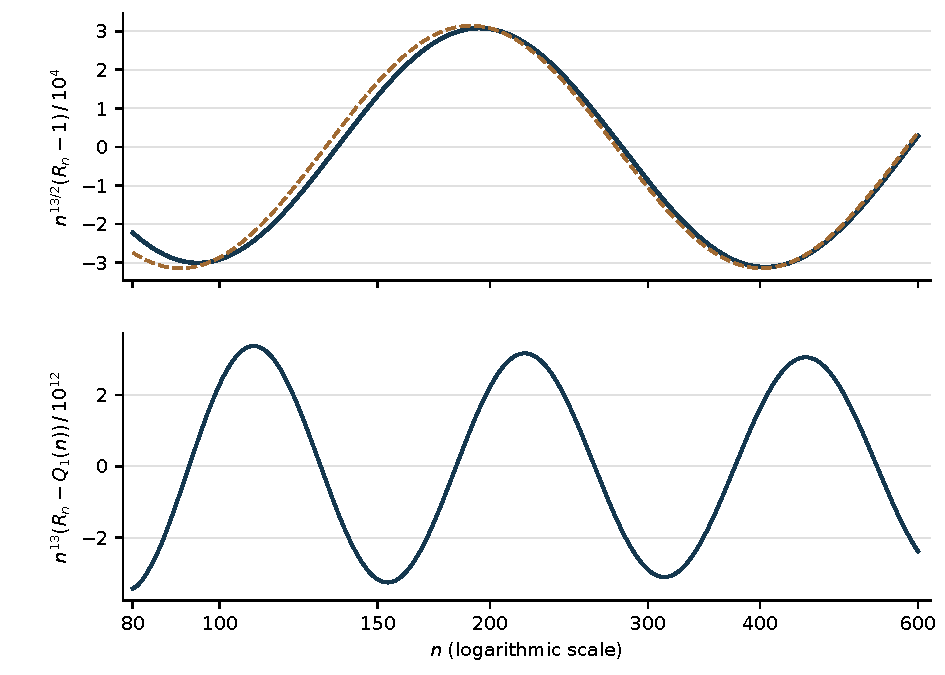
\includegraphics[width=\linewidth]{figures/oscillation.pdf}
\caption{Exploratory illustration using exact counts for every integer $80\le n\le600$ and the fitted constants in \eqref{eq:rho-numeric}. The upper panel shows the logarithmically oscillating normalized discrepancy (solid) and its leading cosine (dashed). The lower panel scales the residual after the exact first Gamma-ratio correction by $n^{13}$. The figure illustrates the proven orders but does not certify the constants or a uniform numerical bound.}\label{fig:oscillation}
\end{figure}

Finite-$n$ error is not necessarily monotone in truncation degree, particularly at small indices. Near a zero of an oscillatory term, the error can also look unusually small. At very high grades, uncertainty in the fitted constants sets a floor. These effects are consistent with a fixed-grade theorem and should not be presented as failures or numerical proofs of its asymptotic remainder.

The inverse replay evaluates exact thresholds $X=h_n$ and geometric midpoints $X=\sqrt{h_nh_{n+1}}$ for $n=75,100,150,200$. Midpoint ceilings agree with the exact inverse in all four tests. At thresholds, tiny signed errors in the continuous root demonstrate why an unconditional ceiling claim would be unsafe. The code labels these computations as exploratory.

\subsection{How to replay and rebuild}
From the extracted archive root, the two principal commands are
\begin{quote}\ttfamily
 bash replay.sh\par
 bash build.sh
\end{quote}
The first uses Python~3 with \texttt{mpmath}, \texttt{sympy}, and \texttt{scipy}; it runs in an isolated output directory, preserving the shipped data, and produces a comparison summary and environment information. The replay reruns both precision fits, the original exact and inverse checks, the fourth-order supplement, and the uniform high-order certificates. The report figure can be regenerated from the supplied exact counts and fitted data with \texttt{make\_figure.py}; this additionally needs \texttt{matplotlib}.

The second uses pdfLaTeX and BibTeX. If the TeX installation has its package tree but lacks a prebuilt format or standard font map, the script creates the missing format and map inside the package-local \texttt{.build} directory. It does not change the system TeX installation. The build fixes the source date for stable PDF metadata. A manifest records the released file hashes; check it before replay with \texttt{sha256sum -c MANIFEST.sha256}. Reproducibility of exact data is byte-for-byte. Floating-point comparisons are reported separately, and cross-platform last digits are not claimed to be invariant.

\section{Scope and further questions}
\subsection{What has been established}
The $m=2$ and $m=3$ instances of the published coefficient conjecture hold, with nonzero oscillatory corrections, convergent local expansions, all fixed coefficient grades, and qualified eventual inverses. Every instance with $m\ge29$ is false for its specified all-one sequence. These results leave the intervening orders unresolved here, make no claim that $29$ is the first failing parameter, and do not settle the separate even-order historic-tree Conjecture~2.

The journal's Table~1 is headed by $\rho_m^{-1}$ but lists $3.7746$ at $m=2$. Under its definition of $\rho_m$ as the positive singularity, the independent recurrence and ODE computations agree with that number as the radius rather than its reciprocal. This appears to be a reciprocal-label error. The intrinsic definition \eqref{eq:rho} and analytic bounds \eqref{eq:rho-bounds} remove any dependence on that convention.

A bounded source check on 2 October 2026 considered the primary journal paper, its predecessor, accessible OEIS records, the cited Emden--Fowler literature, B-urns, and relevant public repository searches. It located no prior resolution of the specific counting statements presented here. That is a bounded negative finding, not an exhaustive priority certificate. The real-axis results, underlying spectral family, sign-regularity results, linearization, and transfer methods are explicitly credited.

\subsection{Questions that follow naturally}
\begin{enumerate}
 \item \textbf{The actual high-order asymptotic.} What replaces the proposed factorial-pole equivalent for $m\ge29$? The nonconvergence result alone does not distinguish periodic profiles, more complicated bounded behavior, or other possibilities. Any claim about a periodic limit needs an additional global dynamical argument.
 \item \textbf{The intervening orders.} Which of the cases $4\le m\le28$ satisfy the conjectured equivalent? The exact spectral check at ODE order $29$ removes one particular local instability, but local spectral stability does not prove that the selected orbit enters the equilibrium's basin. Is $m=29$ actually the first failure?
 \item \textbf{Certified constants and thresholds.} Can validated integration, effective linearization bounds, and quantitative Delta domains give interval enclosures for the low-order radii and amplitudes, and explicit finite-$X$ inverse brackets? This would make the asymptotic inverse statements directly usable for certified integer recovery.
 \item \textbf{Global singularities and effective convergence.} Quantitative majorants could make the local bidisk or tridisk radius explicit. Locating more distant complex singularities could also identify contributions beyond every fixed algebraic order; local analyticity of diagonal terms is insufficient for such a claim.
 \item \textbf{Broader initial data and combinatorial meaning.} The cone argument suggests studying other positive jets with log-concave normalized coordinates. Separately, is there a direct interpretation of the low-order logarithmic oscillations in the evolution of B-tree histories, beyond the nonlinear ODE and its focus eigenvalues?
\end{enumerate}

\appendix
\section{A compact verification guide}
The detailed third-order proof dependencies can be checked in the following order.
\begin{enumerate}
 \item Verify the change of variables \eqref{eq:coordinates} and the exact cancellation in \eqref{eq:Vdot}. Compactness must allow the harmless boundary $p=0$, while keeping $q$ away from zero.
 \item Reconstruct the real solution by \eqref{eq:reconstruction}. Finite $\rho$ and the constant $60$ follow without a numerical approximation.
 \item Check the nonresonant Poincar\'e hypotheses for \eqref{eq:jacobian}; a smooth or formal linearization would not suffice for the claimed convergence.
 \item Check the signs in \eqref{eq:S} and \eqref{eq:w}, then the exact time identity \eqref{eq:time-exact}. The coefficient denominators in $S$ and $B$ have real parts growing with total degree.
 \item Apply analytic implicit inversion at $(\mathcal R,\eta)=(1,0)$, where the derivative is $1$. Nonzero orbit constants and \eqref{eq:linearcoeff} prove $C\ne0$.
 \item Separate the proof of the radius from the proof of uniqueness on the circle. Strict positivity for each of $H,H',H''$ gives the common margin in \eqref{eq:strict} and the dominating disk \eqref{eq:disk}.
 \item Transfer finitely many terms only. Remove analytic diagonal monomials, retain exact Gamma ratios, and expand one extra grade to justify the noninteger-tail remainder.
 \item Invert the logarithmic expansion using monotonicity and a ceiling window. Neither fitted constants nor a root extremely near an integer justify dropping that window.
\end{enumerate}

For the fourth-order result, additionally check the monotone-density derivative upgrade, the three nonresonant exponents, the conserved energy, and the backward-Metzler exclusion of a pure real mode. For the uniform obstruction, verify the finite rational phase bounds and the infinite-range inequalities, the whole-subspace sign-variation theorem, and the generalized stable-manifold hypotheses. The last step must use the slow/fast spectral gap; ordinary hyperbolic stability alone would not cover every high order.

\bibliographystyle{plain}
\bibliography{references}
\end{document}
